\documentclass[11pt,letterpaper]{article}

\usepackage{amsmath}
\usepackage{amsfonts}
\usepackage{amssymb}
\usepackage{makeidx}
\usepackage{graphicx}
\usepackage[left=1.00in, right=1.00in, top=1.00in, bottom=1.00in]{geometry}
\usepackage{epstopdf}


%% Mathematical options & shortcuts

% A fix for parentess
\delimitershortfall=-1pt


% Required packages
\usepackage{ifthen}
\usepackage{mathtools} % Required for nice conditional expectation operator


% Widebar hack - due to 
\makeatletter
\newcommand*\rel@kern[1]{\kern#1\dimexpr\macc@kerna}
\newcommand*\widebar[1]{%
	\begingroup
	\def\mathaccent##1##2{%
		\rel@kern{0.8}%
		\overline{\rel@kern{-0.8}\macc@nucleus\rel@kern{0.2}}%
		\rel@kern{-0.2}%
	}%
	\macc@depth\@ne
	\let\math@bgroup\@empty \let\math@egroup\macc@set@skewchar
	\mathsurround\z@ \frozen@everymath{\mathgroup\macc@group\relax}%
	\macc@set@skewchar\relax
	\let\mathaccentV\macc@nested@a
	\macc@nested@a\relax111{#1}%
	\endgroup
}
\makeatother




% Fixing quotation - must use "etoolbox"
%\newtoggle{quotopen}
%\toggletrue{quotopen}
%%\catcode34=\active % lets you define `"` as a macro
%\DeclareRobustCommand{\testme}{%
%	\iftoggle{quotopen}{%
%		\togglefalse{quotopen} 
%		``
%	}{%
%	    \toggletrue{quotopen} ''
%	}
%}
% Deactive with: \catcode`\"=12\relax % changes `"` back to normal





% Equations referencing:
\newcommand{\Eq}[1]{Eq.~\eqref{eq:#1}\xspace}
\newcommand{\Eqs}[1]{Eqs.~\eqref{eq:#1}\xspace}

% Text related
\newcommand{\etal}{\textit{et al.}\xspace}
\newcommand{\apriori}{\textit{a priori}\xspace}
\newcommand{\aposteriori}{\textit{aposteriori}\xspace}
\newcommand{\eg}{\textit{e.g.}\xspace}
%\newcommand{\ie}{\textit{i.e.}\xspace}
\newcommand{\ie}{{i.e.}\xspace}
\newcommand{\etc}{\textit{etc}\xspace}

% Macros
\newcommand{\explain}[2]{\underset{\substack{\uparrow \\ \texttt{#2}}} {#1} } 


% Operators 
\newcommand{\dfn}{\triangleq}
\DeclareMathOperator{\prob}{Prob}
\DeclareMathOperator{\sign}{Sgn}


\DeclareMathOperator{\var}{Var}
\newcommand{\cov}{\mathsf{Cov}}

\DeclareMathOperator{\Jac}{J}
\newcommand{\Order}{\mathcal{O}}

\newcommand{\dOp}{\mathrm{d}}

% Refining forall operator
\let\oldforall\forall
\renewcommand{\forall}{\ensuremath{\; \oldforall \;}}




% Refining SUM operator
%\newcommand{\Sum}[0]{\sum\limits}
\newcommand{\Sum}[3]{\sum\limits_{#1}^{#2} {#3} \hspace{2pt}}

% Refining PROD operator
\newcommand{\Prod}[3]{\prod\limits_{#1}^{#2} {#3} \hspace{2pt}}

% Gradient (nabla) operator
\newcommand{\Grad}[2]{\nabla_{#1}{#2} \hspace{2pt}}

% Integral operator
\newcommand{\Int}[4]{\int\limits_{#1}^{#2}\hspace{-5pt} {#3} \hspace{2pt} \dOp{#4}\hspace{2pt}}


% A nicer transpose
%\DeclareMathOperator{\Transp}{T}
\newcommand{\TR}{{\hspace{-1pt}{\top}\hspace{-1pt}}}






% Symbols
%\newcommand{\diag}[1]{\mbox{diag}\bigl\{#1\bigr\}}
\newcommand{\diag}[1]{\mbox{diag}\left\{#1\right\}}
%\newcommand{\normal}[1]{\mathcal{N}\bigl(#1\bigr)}
\newcommand{\normal}[1]{\mathcal{N}(#1)}
\newcommand{\uniformal}[1]{\mathcal{U}\bigl[#1\bigr]}


%    Enclose the argument in vert-bar delimiters:
\newcommand{\envert}[1]{\left\lvert#1\right\rvert}
\let\abs=\envert
%
%    Enclose the argument in double-vert-bar delimiters:
\newcommand{\enVert}[1]{\left\lVert#1\right\rVert}
\let\norm=\enVert

% Norm of the vector/matrix
\newcommand{\Norm}[2][]{\enVert{#2}_{#1}}


% Vectors & Matrices
%\newcommand{\vc}[1]{}  %vector-matrix in BOLD
%\newcommand{\vc}[1]{#1}  %vector-matrix in BOLD
%\newcommand{\vc}[1]{\mathbold{#1}}  %vector-matrix in BOLD
%\renewcommand{\vec}[1]{\ensuremath{\boldsymbol{#1}}}
%\newcommand{\mtx}[1]{\ensuremath{\boldsymbol{#1}}}

% Prof. Tsiotras request - vectors & matrices are NOT BOLD
\renewcommand{\vec}[1]{\ensuremath{{#1}}}
\newcommand{\mtx}[1]{\ensuremath{{#1}}}



\newcommand{\func}[1]{#1}



% Braces
\newcommand{\br}[1]{{\hspace{-1pt}\left({#1}\right)}}
%\newcommand{\br}[1]{{\hspace{-1pt}(#1)}}
\newcommand{\brs}[1]{{\left[{#1}\right]}}
\newcommand{\brf}[1]{{\left\{{#1}\right\}}}

% Neglected order in linearizations:
\newcommand{\OfOrder}[1]{\Order\brf{#1}}

% Statistics:\
\newcommand{\Expectation}[1]{\mathbb{E}[#1]}
%\newcommand{\Expectation}{\E\expectarg}
%\DeclarePairedDelimiterX{\expectarg}[1]{[}{]}{%
%	\ifnum\currentgrouptype=16 \else\begingroup\fi
%	\activatebar#1
%	\ifnum\currentgrouptype=16 \else\endgroup\fi
%}
%
%\newcommand{\innermid}{\nonscript\;\delimsize\vert\nonscript\;}
%\newcommand{\activatebar}{%
%	\begingroup\lccode`\~=`\|
%	\lowercase{\endgroup\let~}\innermid 
%	\mathcode`|=\string"8000
%}


\newcommand{\ExpectationOver}[2]{\E_{#1}\brs{#2}}



\newcommand{\Cov}[1]{\cov\brs{#1}}
\newcommand{\Var}[2][]{\var_{#1}{#2}}                   % Central Moment 

% Fields
%\newcommand{\field}[1]{\:\mathbb{R}^{#1}}
%\newcommand{\Rfield}{\:\mathbb{R}}
%\newcommand{\Sfield}[1]{\:\mathbb{S}^{#1}}
\newcommand{\domain}[1]{\mathcal{#1}}
\newcommand{\Rfield}{\mathbb{R}}
\newcommand{\field}[1]{\Rfield^{#1}}
\newcommand{\Sfield}[1]{\:\mathbb{S}^{#1}}

\newcommand{\Cone}{\mathcal{C}^{1}}
\newcommand{\Ltwo}{\mathcal{L}_{2}}



\newcommand{\Reals}[1]{\field{#1}}
\newcommand{\Integers}[1]{\mathbb{Z}{#1}}

% Linear algebra
\DeclareMathOperator{\rank}{Rank}
\DeclareMathOperator{\nullity}{Nullity}

\newcommand{\rangespace}[1]{ \mathscr{R}\brf{#1} }
\newcommand{\nullspace}[1]{ \mathscr{N}\brf{#1} } 
\newcommand{\image}[1]{ \mathscr{I}\brf{#1}} 
\newcommand{\Rank}[1]{ \rank\brf{#1}}
\newcommand{\Nullity}[1]{ \nullity\brf{#1}}

\newcommand{\Jmat}[2]{\mtx{J}^{{#1},{#2}}}


% Sets
\newcommand{\given}{\ensuremath{ \ | \ }}




% Kronecker delta
\newcommand{\KronDelta}[1]{\delta_\br{#1}}



% Neighbouhood (ball)
\newcommand{\Ball}[2][]{{\mathrm{B}_{#1}}\br{#2}}
\newcommand{\nhd}{neighbourhood}





%%%%%%%%%%%%% ROTATIONS KINEMATICS %%%%%%%%%%%%%%%
% Cross Matrix 
\newcommand{\xMat}[1]{\brs{#1\times}}

% Euler Rotations
\newcommand{\rotX}[1]{\brs{#1}_x}
\newcommand{\rotY}[1]{\brs{#1}_y}
\newcommand{\rotZ}[1]{\brs{#1}_z}

% DCM from X to Y frames: usage \DCM{x}{y}
\newcommand{\DCM}[2]{\mtx{T}^{#1}_{#2}}
%%%%%%%%%%%%%%%%%%%%%%%%%%%%%%%%%%%%%%%%%%%%%%%%%%



%%%%%%%%%%%% General Math %%%%%%%%%%%%%%%
% Jacobian of vector1 to vector2 
%\newcommand{\jacvv}[3]{ \frac{\partial \vec{#1}}{\partial \vec{#2}} {\br{#3}}}
%\newcommand{\jacvv}[3]{\nabla_{\vec{#2}} \vec{#1}^T {\br{#3}}}
%\newcommand{\Jacobian}[3]{ \left. \brs{\nabla_{#2} {#1}^T}^T \right|_{#3}}

\newcommand{\Jacobian}[4][]{ \Jac^{#1}_{#3} \brf{{#2}\br{#4}} }




% Jacobian of var1 to var2
\newcommand{\jac}[3]{ \frac{\partial #1}{\partial #2} {\br{#3}}}

% Pardial derivative shortcut
\newcommand{\pder}[2]{ \frac{\partial{#1}}{\partial{#2}}}


% Full time derivative
\newcommand{\ddt}{\frac{\dOp}{\dOp t}}


% BMATRIX shortcut
\newcommand{\bmat}[1]{\begin{bmatrix} #1 \end{bmatrix}}


% Inverse
\newcommand{\inv}[1]{{#1}^{-1}}
\newcommand{\invb}[1]{\br{#1}^{\hspace{-2pt}-1}}



% Generic functions
\newcommand{\fun}[2]{#1\br{#2}}
\newcommand{\Dfun}[3]{{#1}_{#2}\br{#3}}
\newcommand{\DfunS}[4]{{#1}^{#2}_{#3}\br{#4}}


%%%%%%%%%%%%%%%%%%%%%%% Generic variables & vectors %%%%%%%%%%%%%%%%%%%%%%%



\newcommand{\funh}[0]{\fun{h}}
\newcommand{\fung}[0]{\fun{g}}

\newcommand{\funfb}[1]{\funf\br{#1}}
\newcommand{\funhb}[1]{\funh\br{#1}}
\newcommand{\fungb}[1]{\fung\br{#1}}



\newcommand{\I}[0]{\mathsf{I}}



%%%%%%%%%%%%%%%%% UNITS %%%%%%%%%%%%%%%%%%%%%
\newcommand{\rad}[0]{\,\texttt{rad}}
\newcommand{\mrad}[0]{\,\texttt{mrad}}
\newcommand{\radsec}[0]{\,\frac{\texttt{rad}}{\texttt{sec}}}
\newcommand{\radsecsec}[0]{\,\frac{\texttt{rad}}{\texttt{sec}^2}}
\newcommand{\mradsec}[0]{\,\frac{\texttt{mrad}}{\texttt{sec}}}

\newcommand{\meter}[0]{\,\texttt{m}}
\newcommand{\msec}[0]{\,\frac{\texttt{m}}{\texttt{sec}}}
\newcommand{\msecsec}[0]{\,\frac{\texttt{m}}{\texttt{sec}^2}}
%%%%%%%%%%%%%%%%%%%%%%%%%%%%%%%%%%%%%%%%%%%%%



%%%%%%%%%%%%% Vector spaces %%%%%%%%%%%%%%
\newcommand{\vecspace}[1]{\mathcal{#1}}


% % % % % % % % % % % % % % % % Shortcuts % % % % % % % %
\newcommand{\half}{\frac{1}{2}}


%% Matrix calculus
\DeclareMathOperator{\Tr}{Tr}
\DeclareMathOperator{\VecOp}{vec}
% Symbols & function
\newcommand{\Det}[1]{|#1|} % Determinant
\newcommand{\Trace}[1]{\Tr\brs{#1}} % Trace
\newcommand{\VecFun}[1]{\VecOp\br{#1}}


% Commutation matrix for some matrix
\newcommand{\CommutMat}[1]{\mtx{T}_{#1}}
\newcommand{\CommutInvMat}[1]{\widetilde{\mtx{T}}_{#1}}

% Kronecker product
\newcommand{\Kron}[2]{\br{{#1} \otimes {#2}}}


% Arcmin






\endinput
%%% Local Variables: 
%%% mode: latex
%%% TeX-master: "main"
%%% End: 


\newcommand{\SNR}{\mathrm{SNR}}


\author{Maxim Golsshtein}
\title{Using a SNRFitting a finger motion with harmonics}
\begin{document}
	\maketitle
	
	\section{Theory}
	
	One of the methods to classify a signal as one that originates from a cyclic motion is to evaluate it's fit to a series of harmonics. In general, any periodic signal with a given frequency $\omega$ can be represented using the Fourier series. Given an infinitely-differentiable bounded function $x(t) = x(t+\frac{2\pi n}{\omega})$ for $t\in\Reals{}$ and $n\in\Integers{}$, there exists $N>0$ for which 
	\begin{equation}\label{key}
	x(t) = a_0 + \sum_{p=1}^{N} a_p \sin(\omega p t) + b_p \sin(2\pi f p t).
	\end{equation}
	where $a_0 \in \Reals{}$, $a_p \in \Reals{}$ and $b_p \in \Reals{}$ for $p \in [1, ..., N]$ are parameters of the Fourier series.
	
	Let $y(t)$ be a measurement of a periodic signal $x(t)$. The measurement includes noise, imperfections in the repetition on the signal, and other measurement artifacts, denoted as $n(t)$:
	\begin{equation}\label{key}
	y(t) = x(t) + n(t)
	\end{equation}
	We model $n(t)$ as a zero-mean random process, with a variance $\sigma_n^2$.
	
	A signal-to-noise ratio (SNR) is defined as a ratio between the power of the signal and the power of the noise. For periodic signals and zero mean uncorrelated random noise, this ratio is: 
	\begin{equation}\label{key}
		 \SNR \dfn \frac{\sigma_x^2}{\sigma_n^2}
	\end{equation}
	where 
	\begin{equation}\label{key}
		\sigma_x^2 = \half\sum_{p=1}^{N} a_p^2 + b_p^2.
	\end{equation}
		
	For sufficiently large periodic motion, the SNR will be larger than a specified threshold, and can be used to classify the signal. 
	
	\section{Solution}
	
	In order to calculate the SNR, the measured signal must first to be divided into the signal and the noise parts. Suppose the signal have been measured for several periods periods: $y(t_i)$, $i=0,...,m$, where $i \in \brf{i: 0 \leq t_i < 1/f}$ are the indexes of the first period time samples, $i \in \brf{i: 1/f \leq t_i < 2/f}$ are of the second period, and so on.
	We assume that signal contains a slow-changing bias $b(t_i)$, which is approximately constant during each period. This bias can be approximated by taking an average of the samples during each period, or by filtering the signal with a very-low-bandwidth low-pass filter.
	In addition, the signal is assumed to contains $N$ significant harmonics, such that $2N < m$, and the measured noise/artifacts are uncorrelated at each sample.
	
	Let $A\in\Reals{m \times 2N}$ be the measurement matrix:
	\begin{equation}
	A = \bmat{ \sin(\omega t_0) & \cos(\omega t_0) & \sin(2 \omega t_0) & \cos(2 \omega t_0) & \cdots & \sin(N \omega t_0) & \cos(N \omega t_0) \\
		\sin(\omega t_1) & \cos(\omega t_1) & \sin(2 \omega t_1) & \cos(2 \omega t_1) & \cdots & \sin(N \omega t_1) & \cos(N \omega t_1) \\
		\vdots &  &  & \vdots &  &  & \vdots \\
		\sin(\omega t_m) &  &  & \cdots &  & & \cos(N \omega t_m)
		},
	\end{equation}
	and let $\phi \in \Reals{2 N}$ be a vector of the Fourier series parameters:
	\begin{equation}
		\phi = \bmat{a_1 & b_1 & a_2 & b_2 & \cdots & a_N & b_N}^{\TR}.
	\end{equation}
	%
	The measurement set can be represented as:
	\begin{equation}\label{eqMsrSetRepresentation}
	\underbrace{\bmat{y(t_0) \\ \vdots \\ y(t_m)}}_{\dfn Y} - \underbrace{\bmat{b(t_0) \\ \vdots \\ b(t_m)}}_{\dfn B} = A \phi + \underbrace{\bmat{n(t_0) \\ \vdots \\ n(t_m)}}_{\dfn r}
	\end{equation}
	
	The best fit of the parameters to the signal, that maximizes the SNR, is given by a least-squares solution of the equation~\eqref{eqMsrSetRepresentation}:
	\begin{equation}\label{eqLSsolution}
	\widehat{\phi} = \invb{A^{\TR} A} A^{\TR} (Y - B).
	\end{equation}
	The noise is estimated as the estimation residual:
	\begin{equation}\label{key}
	\widehat{r} = \br{\I - \invb{A^{\TR} A} A^{\TR}}(Y - B),
	\end{equation}
	and the SNR is estimated using the sample covariance:
	\begin{equation}\label{key}
	\widehat{\SNR} = \frac{m-1}{2} \frac{\Norm[2]{\phi}^2}{\Norm[2]{r}^2}
	\end{equation}
	
	\section{Numerical Example}
	Figures~\ref{figXaxisMagSignalWalkingSync} and~\ref{figXaxisMagSignalWalkingNoise}  exhibits two signals, measured by the $x$ axis of the smartwatch magnetometer. One signal was recorder while the user was trying to sync their magnetic ring-wearing finger motion with the (user presented) periodic ($\frac{2\pi}{omega} = 0.75s$) signal. The second set was recorded during the user's normal activity (walking). After 4 seconds from the start, the harmonic signal was extracted, using $N=2$ and 5 full periods. The figures show the signal and the fitted periodic wave. Using the estimated SNR, the finger-motion-induced signal can be clearly identified. 
	
	\begin{figure}[tbph]
		\centering
		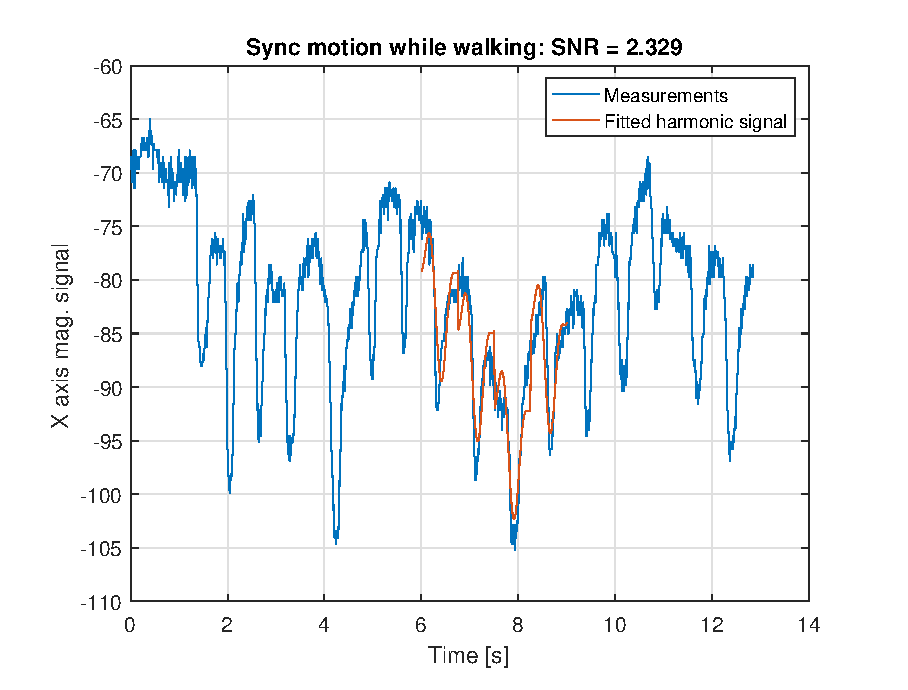
\includegraphics[width=0.8\linewidth]{WalkSig}
		\caption{Signal recorder while walking and syncing.}
		\label{figXaxisMagSignalWalkingSync}
	\end{figure}
	\begin{figure}[tbph]
		\centering
		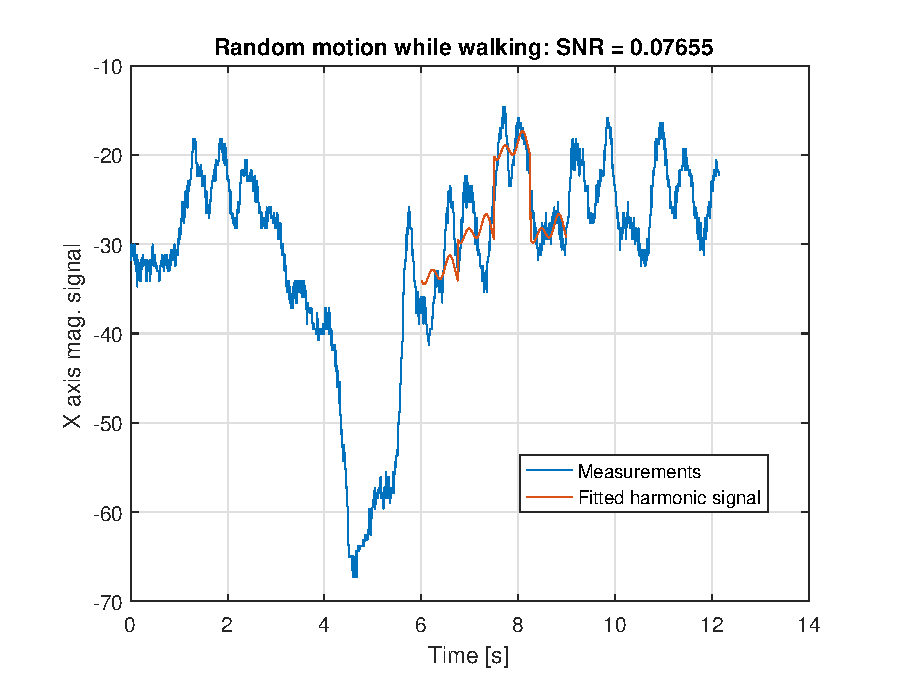
\includegraphics[width=0.8\linewidth]{WalkNoise}
		\caption{Signal recorder while walking (random motion).}
		\label{figXaxisMagSignalWalkingNoise}
	\end{figure}
	
	
	
	
	
	
	
	
	
	
	
	
	
	
\end{document}